This section will investigate the influence of the shape of the re-entry vehicle on several important design parameters, as well as the sensitivity of these parameters to changes in vehicle shape. It will start by identifying the most important design parameters. This will be followed by a section discussing which shapes will generate a local optimum for a single design parameter. The knowledge of these single parameter optima will be used in the final section to discuss the total set of design parameters for various vehicle shapes. 


\paragraph{Important parameters}
 The following parameters were determined to have a significant influence on te performance of the vehicle:

\begin{itemize}
	\item{Lift. As detailed in section \ref{subsec:controlsens}!!CHECK REFERENCE!! (?), the vehicle requires a lift vector to provide flight path control. A larger lift vector provides an increase in flight path control.}
	\item{Drag. The vehicle decelerates purely on atmospheric drag. An increase in drag will decrease the required time for re-entry and provides greater flexibility in terms of the path through the atmosphere. }
	\item{Lift to Drag ratio. The lift to drag is an indication of the freedom in the selection of the orbital trajectory. A higher lift to drag ratio will provide greater flexibility.}
	\item{\gls{sym:cm-alpha}. The derivative with respect to angle of attack of the moment coefficient is a measure of the stability of the vehicle. }
	\item{\gls{cg} offset}. The \gls{cg} offset at a given angle of attack required to cancel the moment generated by the vehicle at that angle of attack. It is a measure of the control effort required to trim the vehicle. 
	\item{Heat flux. For a given flight condition, the heat flux in the stagnation point depends only on the vehicle geometry.  }
\end{itemize}


\paragraph{Shape sensitivity} \label{sec:aerooptima}
Obtaining favourable characteristics of the aerodynamic shapes requires understanding of the influence of shape parameters on the performance of the design. To this end, firstly an analytical approach is taken. After that, conclusions can be made about different aerodynamic shapes. The optimisation tool is used afterwards to generate shapes that are optimised for certain design parameters, such that the conclusions based on the analytical knowledge can be verified.

In Figure \ref{fig:ldplot}, the lift and drag performance as well as the lift over drag ratio of a flat plate in a free stream is given. Since Newtonian flow theory is based on the assumption that pressure only depends on the local body incidence angle, this plot can be used to deduce performance of a given shape. As can be seen in the plot, a vehicle with a high drag has most of it's surface perpendicular of the flow.

\paragraph{Lift}
A high lift is achieved by having large parts of the shape under an incidence angle of $35 [^\circ]$. An axisymmetric shape doesn't create lift at zero angle of attack, since every radial part of the shape cancels all non-drag forces out. Skewness of the shape, such as portrayed in Figure \ref{fig:skewnessplot}, can be used to create lift at zero angle of attack: a larger part of the surface is inclined upwards than downwards, meaning the skewed shape generates a downward lift. Using skewness instead of an axisymmetric body at a high angle of attack may help to prevent the shock wave from hitting the payload module.

\paragraph{Drag}
A high lift over drag ratio is found at the highest possible angle of attack for a flat plate.

\paragraph{Lift over drag}
A high lift over drag is achieved by having the highest angle of attack for every part of the spacecraft. This entails having a flat plate at the maximum angle of attack for maximum lift over drag. If a non-flat body is chosen, large parts of the area should be nearly under a high inclination, which can be realised by having a very long body at a small angle of attack.

\paragraph{Static stability}
The aerodynamic shape required for static stability can be argued based on the local inclination angle. The pressure force always acts normal to the surface. A large moment arm can be created by inclining the outer edges of the aeroshell. At a positive angle of attack, the lower edge of the aeroshell is turned more perpendicular to the flow such that its pressure force is increased. An example of a shape that features this is given in Figure \ref{fig:skewnessplot}. Depending on the location of the \acrfull{cg}, at an angle of attack the lower part pressure is increased while the pressure on the upper part is decreased, generating a moment. This means that for an increase in angle of attack, the restoring moment is also increased.

\paragraph{Center of gravity shift}
In order to trim the aeroshell at a certain angle of attack, a \gls{cg} offset is used: the \gls{cg} does not lie directly on the most forward point of the spacecraft. In order to minimise the impact, the required \gls{cg} offset is calculated using Equation \ref{eq:reqcgoffset}. A large offset may be unrealistic and more difficult to implement.

\begin{equation} \label{eq:reqcgoffset}
z_{\gls{cg}} = \frac{\gls{sym:CML}}{\gls{sym:CL}}
\end{equation}
In general the relation between required \gls{cg} offset for a certain lift over drag ratio is a good indicator for the performance of a design, since this relates the performance to the cost of the performance.

Finally, the heat flux is given in Equation \ref{eq:modnewtonianqw} and is directly dependent on the density and velocity as well as the local radius of curvature. A less curved body in the stagnation point thus leads to a lower heat flux.


\begin{figure}[h]
	\centering
	\begin{subfigure}[b]{0.48\textwidth}
		\centering
		\setlength\figureheight{0.88\textwidth} 
		\setlength\figurewidth{0.88\textwidth}
		% This file was created by matlab2tikz.
% Minimal pgfplots version: 1.3
%
\definecolor{mycolor1}{rgb}{0.00000,0.44700,0.74100}%
\definecolor{mycolor2}{rgb}{0.85000,0.32500,0.09800}%
\definecolor{mycolor3}{rgb}{0.92900,0.69400,0.12500}%
%
\begin{tikzpicture}

\begin{axis}[%
width=0.95092\figurewidth,
height=\figureheight,
at={(0\figurewidth,0\figureheight)},
scale only axis,
xmin=0,
xmax=90,
xlabel={Incidence angle [deg]},
xmajorgrids,
ymin=0,
ymax=2,
ylabel={Relative value},
ymajorgrids,
axis x line*=bottom,
axis y line*=left,
legend style={legend cell align=left,align=left,draw=white!15!black}
]
\addplot [color=mycolor1,solid,mark=o,mark options={solid}]
  table[row sep=crcr]{%
0	0\\
5.72957795130823	0.0988384058270419\\
11.4591559026165	0.190827951047524\\
17.1887338539247	0.269711779072206\\
22.9183118052329	0.330364357068969\\
28.6478897565412	0.369230131302064\\
34.3774677078494	0.384622526068308\\
40.1070456591576	0.376856763471641\\
45.8366236104659	0.348204817862668\\
51.5662015617741	0.302676697465328\\
57.2957795130823	0.245647748216941\\
63.0253574643906	0.183365416479547\\
68.7549354156988	0.122379660668094\\
74.484513367007	0.0689480065583048\\
80.2140913183152	0.0284684893937181\\
85.9436692696235	0.00499121723473934\\
};
\addlegendentry{Relative Lift};

\addplot [color=mycolor2,solid,mark=x,mark options={solid}]
  table[row sep=crcr]{%
0	1\\
5.72957795130823	0.985087246239921\\
11.4591559026165	0.941383837108351\\
17.1887338539247	0.871904858911871\\
22.9183118052329	0.781385184121332\\
28.6478897565412	0.675871221834705\\
34.3774677078494	0.562201187508987\\
40.1070456591576	0.447420114313402\\
45.8366236104659	0.338181603125063\\
51.5662015617741	0.240189440698733\\
57.2957795130823	0.157728605250993\\
63.0253574643906	0.0933271485919668\\
68.7549354156988	0.0475787117739684\\
74.484513367007	0.0191410454184055\\
80.2140913183152	0.00491015184000582\\
85.9436692696235	0.000353951393082256\\
};
\addlegendentry{Relative Drag};

\addplot [color=mycolor3,solid,mark=+,mark options={solid}]
  table[row sep=crcr]{%
0	0\\
5.72957795130823	0.100334672085451\\
11.4591559026165	0.202710035508672\\
17.1887338539247	0.309336249609623\\
22.9183118052329	0.422793218738162\\
28.6478897565412	0.54630248984379\\
34.3774677078494	0.684136808341693\\
40.1070456591576	0.84228838046308\\
45.8366236104659	1.02963855705036\\
51.5662015617741	1.26015821755034\\
57.2957795130823	1.5574077246549\\
63.0253574643906	1.96475965724865\\
68.7549354156988	2.57215162212632\\
74.484513367007	3.60210244796798\\
80.2140913183152	5.79788371548289\\
85.9436692696235	14.1014199471717\\
};
\addlegendentry{Relative Lift/Drag};

\end{axis}
\end{tikzpicture}%
		\caption{Lift, drag and lift over drag ratio for a flat plate versus incidence angle}
		\label{fig:CLCD-incidence}
	\end{subfigure}
	\begin{subfigure}[b]{0.48\textwidth}
		\centering
		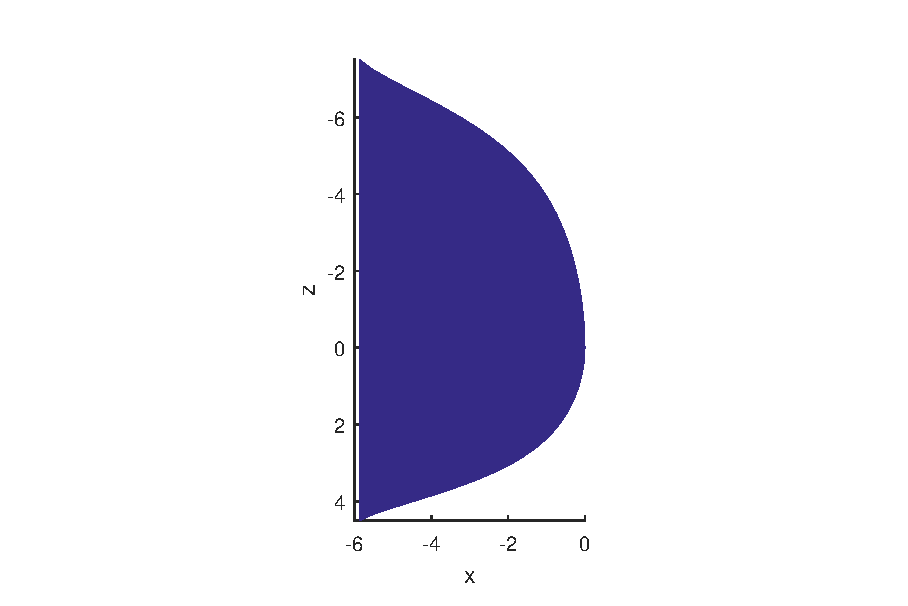
\includegraphics[width=0.9\textwidth]{./Figure/Aerodynamics/skewness.eps}
		\caption{Side-view of a skewed aerodynamic shape. The lower part generates a moment around the frontal part of the aeroshell when under an angle of attack}
		\label{fig:skewnessplot}
	\end{subfigure}
	\caption{}
\end{figure}

To illustrate the characteristics of different aerodynamic shapes, an optimisation has been performed towards certain aerodynamic coefficients, as explained in Paragraph \ref{par:Optimisation}. These shapes serve to enlarge understanding of how certain shape aspects correspond to certain aerodynamic properties. For the following parameters has been optimised:
\begin{itemize}
	\item Drag coefficient \gls{sym:CD}: The maximum drag should be attained by a flat plate at a zero angle of attack. This is also the result of the optimisation towards a maximal drag.
	\item Lift coefficient \gls{sym:CL}: As per the analysis in Paragraph \ref{sec:aeroparams}, the maximum lift coefficient is achieved by a flat plate at an angle of attack of $35^\circ$. This is confirmed by the optimisation algorithm, which produces the same flat plate as for maximum drag, but at an angle of attack.
	\item Lift over Drag $\frac{\gls{sym:L}}{\gls{sym:D}}$: The maximum lift over drag ratio is found for a flat plate at an angle of attack as high as possible. This result was achieved at an angle of attack of $40^\circ$, which is limited to keep the design in the range where the shockwaves don't hit the payload module.
	\item Static stability \gls{sym:cm-alpha}: For this parameter, it is necessary to have large parts of the aerodynamic shape inclined with respect to the flow. The optimisation confirms this and creates a shape as portrayed in Figure \ref{fig:highcmalphashape}. This optimisation was constrained by a maximum length.
	\item \gls{cg} shift $\frac{\gls{sym:CM}}{\gls{sym:CX}}$: The minimum \gls{cg} shift for a given angle of attack is achieved by a flat plate since it generates very little moment. However, if static stability is required, the contours of the aeroshell can be inclined inwards.
\end{itemize}


\begin{figure}
	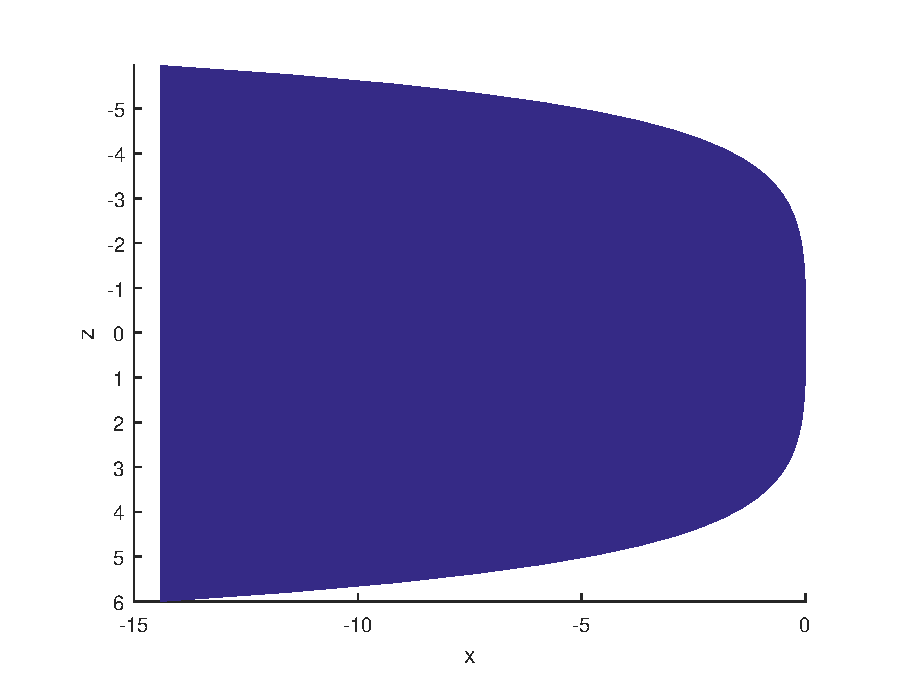
\includegraphics[width=0.9\textwidth]{./Figure/Aerodynamics/cmalphamax.eps}
	\caption{Optimised shape resulting in high static stability}
	\label{fig:highcmalphashape}
\end{figure}
	

\paragraph{Various shapes} \label{sec:aeroshapes}
Several large groups of varying shapes can be identified. Every aeroshell shape can be categorized in one of these groups.  Each group of shapes has advantages and disadvantages. The relative performance of each group can be qualitatively assessed by looking at the variations of the shape with respect to the optimal shapes for the various parameters. The effect of asymmetric cross-sections will be ignored in this assessment, and will be investigated separately. In figure \ref{fig:aeroshapes} representative cross sections of the groups can be seen. Group A represents simple concave surfaces. Group B has a concave centre section with a flat ring around it. Group C has an approximately flat central section, with steep edges around the outer radius. Group D represents the half cone shapes, with relatively straight sides and a blunt nose. 

\begin{figure} 
	\centering
	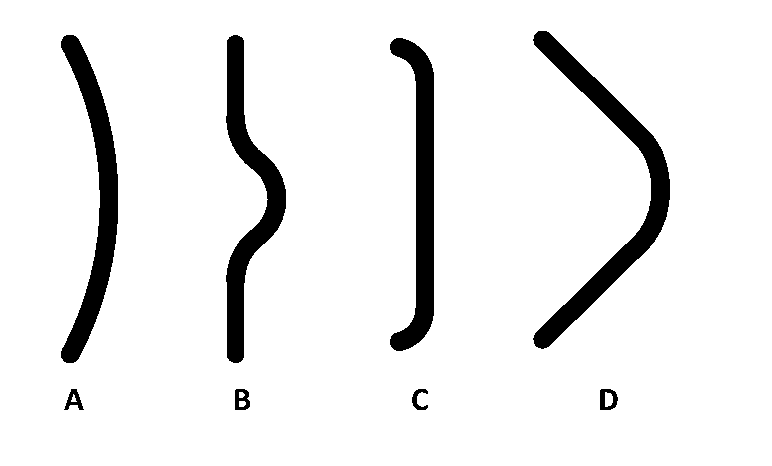
\includegraphics[width=0.5\textwidth]{./Figure/Aerodynamics/AeroShapes.pdf}
	\caption{Various schematic aerodynamic configurations}
	\label{fig:aeroshapes}
\end{figure}

As was discussed in section \ref{sec:aerooptima}, a flat plate will generate the most lift and the most drag, albeit at different angles of incidence. Since Group C closely mimics a flat plate in the majority of its cross-section, it will have the best lift and drag performance. Group B also has a significant flat section and will therefore also have good performance in terms of lift and drag. Groups A and D will both have significant portions of their cross-sections at sub-optimal incidence angles for maximum lift or drag, and will therefore have lower lift and drag performance.

The \gls{sym:cm-alpha} of a given shape is a measure of stability. Shapes which require large moments to change the angle of attack have a higher stability. As can be seen in figure \ref{fig:CLCD-incidence}, surfaces at incidence angles of $40\deg-60\deg$ provide large changes in force for small changes in angle of incidence. Sections at these incidence angles will therefore stabilize the vehicle, since a change in angle of attack will cause one side of cross section to generate a greater moment than the other. This is visualized in figure \ref{fig:StabMom}. Cross sections B and C have parts of their cross section at such angles. Since the sections in C are on the outside of the cross section, it will be significantly more stable than type B due to the moment arm these parts have. A and D will have significant portions of their cross sections contribute to the vehicle moment. Although these section are likely to be at sub optimal angles of incidence for high stability, the large area contributing to the stability of the vehicle will ensure that both types of cross section are stable. 

\begin{figure} 
	\centering
	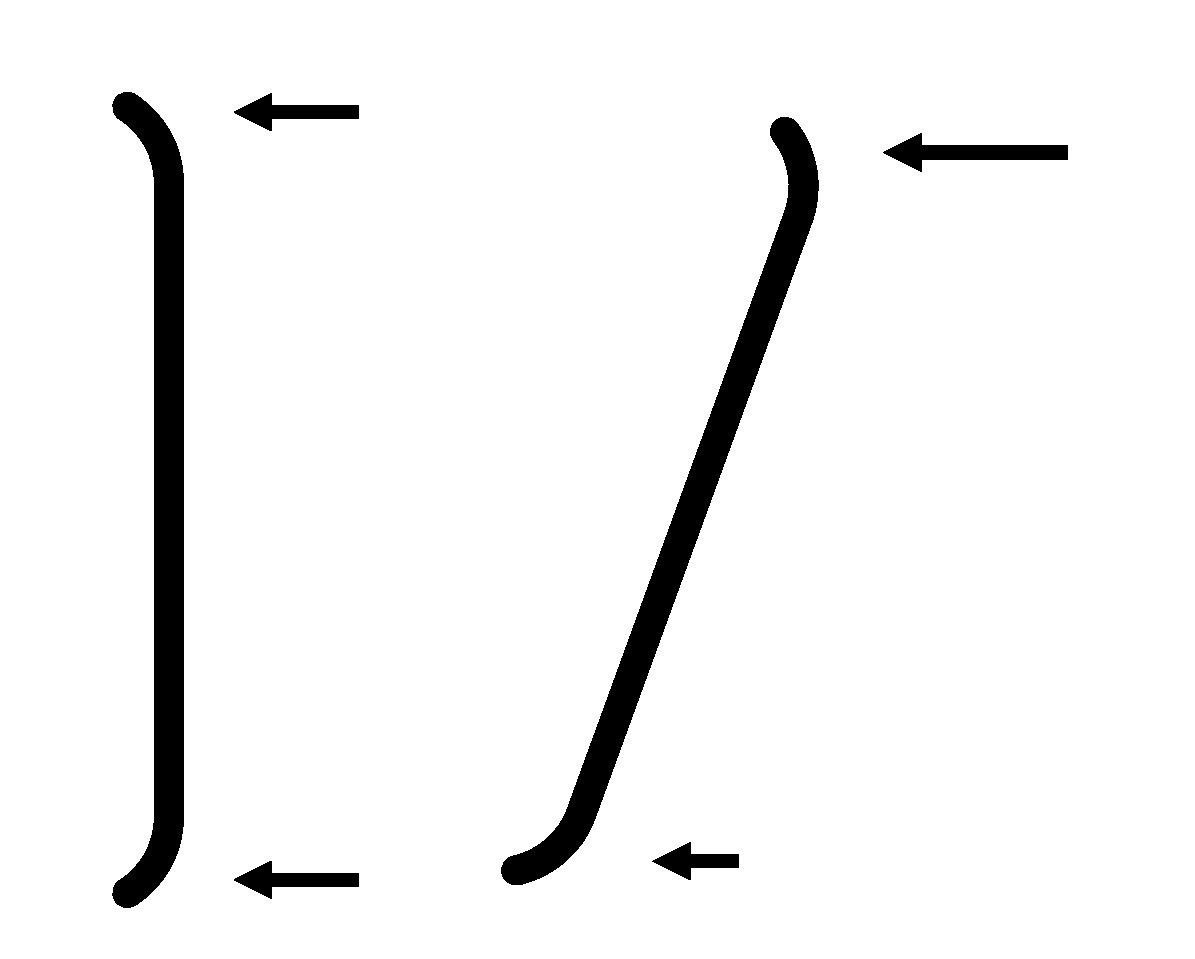
\includegraphics[width=0.5\textwidth]{./Figure/Aerodynamics/StabilizeMoment.pdf}
	\caption{Stabilizing effect of reduced incidence angle sections. }
	\label{fig:StabMom}
\end{figure}

\paragraph{Asymmetry}
An asymmetric body will ensure that even at zero degrees angle of attack, the vehicle generates lift. As explained in section \ref{subsec:orbitsens}, this allows for greater control of the vehicle during re-entry and is therefore desirable. Since the angle of attack that can be attained is limited by, among others, the crew module extending into the flow around the body, achieving high lift at a low angle of attack is a desirable property. The level of asymmetry is also limited by the crew module extending into the flow. If the shape is heavily offset to one edge of the body, the crew module will extend into the flow at very low angles of attack. Figure \ref{fig:LDSkew} shows the effect of asymmetry on the lift to drag ratio by transforming a given symmetric shape into an asymmetric shape. The asymmetric shapes are created by a linearly shifting the cross sections of the body in the $zy$-plane along the $y$-axis, with no shift at $x=0$ and maximum shift at $x=x_{max}$. 

\begin{figure} 
	\centering
	\setlength\figureheight{0.48\textwidth} 
	\setlength\figurewidth{0.88\textwidth}
	% This file was created by matlab2tikz.
% Minimal pgfplots version: 1.3
%
\definecolor{mycolor1}{rgb}{0.20810,0.16630,0.52920}%
\definecolor{mycolor2}{rgb}{0.07947,0.51590,0.83283}%
\definecolor{mycolor3}{rgb}{0.19855,0.72140,0.63095}%
%
\begin{tikzpicture}

\begin{axis}[%
width=0.95092\figurewidth,
height=\figureheight,
at={(0\figurewidth,0\figureheight)},
scale only axis,
xmin=0,
xmax=30,
xlabel={Angle of attack ($\alpha$) [deg]},
xmajorgrids,
ymin=-0.15,
ymax=0.35,
ylabel={$C_{L}C^{-1}_{D}$},
ymajorgrids,
axis x line*=bottom,
axis y line*=left,
legend style={at={(0.97,0.03)},anchor=south east,legend cell align=left,align=left,draw=white!15!black}
]
\addplot [color=mycolor1,solid,mark=o,mark options={solid}]
  table[row sep=crcr]{%
0	2.61154748320994e-17\\
2	0.0417466658947308\\
4	0.0823200861050327\\
6	0.120617408865941\\
8	0.155667575883258\\
10	0.186838218719932\\
12	0.214306384300434\\
14	0.238370040330934\\
16	0.259191095413009\\
18	0.276846062724509\\
20	0.291382695673\\
22	0.302845834113712\\
24	0.311296999304606\\
26	0.31682552065831\\
28	0.319546168484068\\
30	0.319595814761462\\
};
\addlegendentry{No offset};

\addplot [color=mycolor2,solid,mark=x,mark options={solid}]
  table[row sep=crcr]{%
0	-0.0510999775913039\\
2	-0.00924427858967091\\
4	0.0326245851548465\\
6	0.0733275968937169\\
8	0.111754491243533\\
10	0.146973673497436\\
12	0.178763878844936\\
14	0.207305747524724\\
16	0.232680738764875\\
18	0.254888467496611\\
20	0.273894475487587\\
22	0.289675694705614\\
24	0.302232582775283\\
26	0.311605295035817\\
28	0.3178736503127\\
30	0.321152888031585\\
};
\addlegendentry{0.5m offset};

\addplot [color=mycolor3,solid,mark=+,mark options={solid}]
  table[row sep=crcr]{%
0	-0.101551805031846\\
2	-0.0605681572158631\\
4	-0.0183707641330737\\
6	0.0238504964562734\\
8	0.0649014834805692\\
10	0.103662646246088\\
12	0.139492016187436\\
14	0.172382432714766\\
16	0.202317459198565\\
18	0.229199160626968\\
20	0.252895438257389\\
22	0.273289622257361\\
24	0.290297030575286\\
26	0.30388694046641\\
28	0.314087026010277\\
30	0.320975585860611\\
};
\addlegendentry{1m offset};

\end{axis}
\end{tikzpicture}%
	\caption{Effect of asymmetric shape on Lift over Drag ratio }
	\label{fig:LDSkew}
\end{figure}






















